\documentclass[12pt]{article}
\usepackage[margin=1in]{geometry}
\usepackage[T1]{fontenc}
\usepackage{lmodern}
\usepackage{setspace}
\usepackage{amsmath}
\usepackage{booktabs}
\usepackage{threeparttable}
\usepackage{graphicx}
\usepackage[font=small,labelfont=bf]{caption}
\usepackage[authoryear,round]{natbib}
\usepackage{xcolor}
\usepackage[colorlinks=true,linkcolor=black,citecolor=blue!50!black,urlcolor=blue!50!black]{hyperref}
\usepackage{float}
\usepackage{placeins}
\usepackage{needspace}
\usepackage{etoolbox}
\pretocmd{\section}{\FloatBarrier\Needspace{12\baselineskip}}{}{}
\pretocmd{\subsection}{\Needspace{7\baselineskip}}{}{}

\setlength{\bibsep}{3pt}
\begin{document}
\begin{titlepage}
\centering
\vspace*{0.2cm}
{\large WORKING PAPER}\\[1.2cm]
{\Large \textbf{WHERE THE VOTES ARE:\\[4pt] ELECTORAL STRENGTH AND LOCAL SPENDING REQUESTS\\[4pt] IN ITALIAN BUDGET LAWS, 2023--2027}}\\[1.4cm]
{\large Tommaso Landi}\\[4pt]
Sant'Anna School of Advanced Studies and University of Pisa\\[1.2cm]
This version: 26 November 2026 (version 2)\\[0.4cm]
Preliminary draft. Please do not circulate without the author's permission.\\[1.0cm]
\begin{minipage}{0.9\textwidth}\footnotesize\singlespacing
\noindent The research question, the dataset design and the empirical strategy are my own. I thank Riccardo Trezzi (\href{https://underlyinginflation.com}{UnderlyingInflation.com}) for the inspiration behind this project. \textbf{Use of AI.} This paper was produced with the fundamental help of Claude, an AI model developed by Anthropic: it wrote most of the code that downloads and parses the parliamentary files, implemented the estimators, ran the specification searches and drafted much of the text under my direction. I defined the questions, chose the specifications to report, checked the data against the official sources and am responsible for every claim and every error. I disclose this in full because readers should be able to judge the work knowing how it was made; the complete data and replication code will be made public so that every number can be reproduced without trusting either of us. Comments are welcome: \href{mailto:tomsciu@gmail.com}{tomsciu@gmail.com}. This is a preliminary draft; it has not been peer reviewed.\\[6pt]
\textbf{Suggested citation:} Landi, T. (2026). Where the Votes Are: Electoral Strength and Local Spending Requests in Italian Budget Laws, 2023--2027. Working paper, v2, 26 November 2026.\\[4pt]
\copyright{} 2026 Tommaso Landi. All rights reserved. No part of this draft, its data or its code may be reproduced or redistributed without the author's written permission.
\end{minipage}
\end{titlepage}

\begin{center}
\textbf{Abstract}
\end{center}
\begin{quote}\small
I assemble every amendment tabled in the budget committees of both chambers of the Italian Parliament to the five budget laws of the XIX legislature (2023--2027): 24,977 proposals with their first signatory, the signatory's group on the day the bill was examined, the official admissibility ruling and the final outcome. I read each text to identify requests of money for a specific municipality or province and match them to party vote shares in the 2022 general election. Ten extra points of vote share raise the probability that a party tables a local request for a province by 12.2 percentage points (mean 13.4). The gradient survives comparing parties within the same province and budget, which absorbs local need, and 137 of 144 alternative specifications are positive and significant. Within regions, it runs largely through the geography of elected deputies rather than through party-level targeting. It is driven by opposition parties, while the main governing party targets provinces where it is relatively weaker. Outcomes depend on who asks: majority proposals are more often ruled inadmissible, but once admitted they are approved 18\% of the time against 4\% for the opposition.
\end{quote}
\vspace{4pt}
\noindent\textbf{JEL:} D72, H61, H77, R50.\quad \textbf{Keywords:} distributive politics, pork barrel, budget amendments, Italian Parliament, legislative behaviour.

\newpage
\onehalfspacing

\section{Introduction}

Every autumn the Italian government sends Parliament a budget law, and every autumn members of Parliament answer with thousands of amendments. Many are general: they change a tax rate, extend a benefit, refinance a national fund. A visible minority asks for money for a single place, such as a bypass in a provincial town, a theatre, a hospital wing or a school gym. Newspapers call them \emph{marchette} or \emph{mance}; political economists call them pork. They are seldom approved, yet they are tabled in large numbers, carefully signed and often publicised in local media.

This paper asks a simple question: where do these requests go? Classic theories of distributive politics give competing predictions. If parties reward their core supporters, requests should cluster where a party is electorally strong \citep{cox1986}. If they court swing voters, requests should go where elections are close \citep{lindbeck1987,dixit1996}. If what matters is the personal vote of individual legislators, requests should follow the geography of who was elected \citep{golden2008,carozzi2016}. Most of the evidence on these questions uses realised transfers. Realised transfers mix the demands of legislators with the choices of the government, the bureaucracy and the budget constraint. Amendments are cleaner. They record what each legislator \emph{asked for}, in writing and with a date, before anyone decided what to grant.

I build a new dataset of all amendments tabled in the budget committees of the Chamber of Deputies and of the Senate to the five budget laws of the current legislature, from the 2023 budget (December 2022) to the 2027 budget (November 2026). The data cover nine bill readings and 24,977 proposals signed by 543 distinct first signatories. For each proposal I record the first signatory and his or her group at the date of examination, the official admissibility ruling, and the outcome (approved, withdrawn, rejected or never voted). I then read the text to identify requests addressed to a specific municipality or province and the sums involved, and match each party--province pair to the party's vote share in the 2022 general election.

The paper documents five results. First, there is a robust positive association between a party's 2022 vote share in a province and the probability that the party tables a local request for that province. With party-by-budget and region fixed effects, ten additional points of vote share are associated with a 12.2 percentage-point increase in that probability, from a mean of 13.4\% (Table~\ref{tab:main}). The association is not explained by local need: comparing different parties in the \emph{same province and budget}, which absorbs every province-level shock, the estimate is 12.4 points (s.e.\ 1.6). Across 144 specifications that vary the outcome, the sample, the fixed effects and the treatment of large cities, all 144 estimates are positive and 137 are significant at 5\% (Figure~\ref{fig:spec}).

Second, within regions the gradient runs largely through the geography of who was elected. I attribute each party's deputies to provinces through the 2022 list constituencies. Once the number of a party's deputies elected in a province is controlled for, the within-region vote-share coefficient falls from 7.5 to 3.7 points and loses significance, while each additional deputy raises the probability of a request by 9.9 points (Table~\ref{tab:mp}). Across Italy, both matter. This is the pattern predicted by a common-pool view in which individual legislators claim resources for their own constituency \citep{weingast1981,perssontabellini1999}, rather than by a centralised party strategy.

Third, the association is driven by the opposition. Opposition parties (PD, M5S, AVS) ask for money where they are strong, whereas Fratelli d'Italia, the senior governing party, tables more local requests where it is relatively weaker (Table~\ref{tab:het}, Figure~\ref{fig:het}). Fourth, the gradient is steeper in provinces where the 2022 contest between the two coalitions was close, while the interaction with the 2027 budget, the last before the next general election, is imprecisely estimated.

Fifth, what passes depends on who asks. A proposal by a majority legislator is 9.0 points more likely to be approved than one by the opposition, whose base approval rate is 2.9\% (Table~\ref{tab:approval}). Decomposing the process by stage shows that the premium is created at the vote, not at the admissibility filter: majority proposals are \emph{less} often ruled admissible (69.7\% against 78.5\%), but once admitted 17.8\% of them pass against 3.7\% of opposition proposals (Figure~\ref{fig:stages}).

These results speak to three literatures. The first studies the electoral targeting of public spending \citep{cox1986,dixit1996,levitt1997,ansolabehere2006,berry2010}. I add evidence on the \emph{demand} side, at the level of individual proposals, and show that core-voter and swing-voter logics can coexist inside the same Parliament depending on whether a party governs. Because the unit of analysis is the request rather than the transfer, I can separate what legislators ask for from what the government grants, and compare parties inside the same province, which the literature on realised transfers usually cannot do. The second studies Italian distributive politics \citep{golden2008,carozzi2016,bracco2015,brollo2012}, which has focused on transfers to municipalities; I move the lens to the parliamentary stage of the budget. The third concerns legislative behaviour and position-taking \citep{mayhew1974}. The low approval rates suggest that many local amendments are signals to constituents rather than serious attempts to obtain funds, which is consistent with the electoral-connection view. The finding that the within-region gradient runs through elected legislators connects the evidence to the common-pool problem in budgeting \citep{weingast1981,perssontabellini1999} and to the role of individual legislators' constituencies in Italy \citep{carozzi2016}.

The data and an interactive version of every figure are public (Section~\ref{sec:avail}). Section~\ref{sec:background} describes the budget process. Section~\ref{sec:data} introduces the data, Section~\ref{sec:strategy} the empirical strategy, Section~\ref{sec:results} the results and Section~\ref{sec:robust} robustness checks, including a specification curve. Section~\ref{sec:concl} discusses the evidence, including the frequent claim that local spending pays for itself through multiplier effects, and concludes.

\section{Institutional background}\label{sec:background}

The Italian budget law is examined by both chambers under a compressed calendar between late October and the end of December. In recent years the two chambers have alternated in the role of first reader: the Chamber of Deputies examined the 2023, 2025 and 2027 budgets first, the Senate the 2024 and 2026 budgets. In practice, the substantive changes to the government's bill happen in the budget committee of the first chamber (the V Commission at the Chamber, the 5th Commission at the Senate). The second chamber receives a text that the majority treats as closed. Amendments are tabled and sometimes voted, but none is approved, because any change would require a third reading before the 31 December deadline.

Any member can table amendments. The committee chair then rules on admissibility. Two grounds dominate: lack of adequate financial coverage, under the constitutional requirement that new spending be funded, and extraneity of subject matter, because the budget law may only contain provisions with a direct financial effect. Since the number of proposals far exceeds the time available, groups are asked to flag a subset of \emph{segnalati} amendments on which votes are actually taken. Government and rapporteurs table their own amendments, often late in the process and often as reformulations of proposals by majority members. Reformulated texts (\emph{nuova formulazione}, \emph{testo 2}) are what is eventually approved.

Two examples from the data illustrate the range of requests. In the 2027 budget, near-identical amendments signed by members of Forza Italia, the Lega, the PD and Azione/Italia Viva (C.~3174-\emph{bis}, 8.09--8.014) proposed a tax credit for bars and restaurants serving draft beer, five million euro a year, which the press described as a beer bonus;\footnote{L.~Graziani, \emph{Open}, 19 November 2026, \url{https://www.open.online/2026/11/19/manovra-tasso-alcolico-spunta-bonus-forza-italia-birra-spina/}.} an amendment on the excise duty on beer had been approved in the 2025 budget (C.~2112-\emph{bis}, 8.066). In the same 2027 file, two amendments by a PD deputy elected in the list constituency that includes the province of Pistoia asked for 50 and 15 million euro over three years for the roads around Collodi and for the ``places of Pinocchio'' in Pescia (89.010 and 89.011); both were ruled inadmissible as extraneous to the subject of the budget law. The first is a sectoral request replicated across parties, the second a textbook local request by a legislator for his own area. This paper is about the second kind.

Two features of this setting matter for what follows. First, tabling is cheap and observable: a legislator can show a local newspaper that he or she ``asked for'' a road or a grant, whatever the outcome. Second, approval is controlled by the government and the majority leadership, so the mapping from requests to outcomes is informative about the bargaining power of different legislators.

\section{Data}\label{sec:data}

\subsection{Sources}

For the Chamber of Deputies I use the official lists of amendments tabled in the V Commission for each budget bill (C.~643-\emph{bis}, C.~1627, C.~2112-\emph{bis}, C.~2750 and C.~3174-\emph{bis}), which report number, article, first signatory with a unique person identifier, and outcome. Texts come from the full amendment files published in the Commission bulletin when available (2024, 2025 and 2027) and otherwise from the individual amendment pages (2023 and 2026). For approved amendments in 2025 I use the text of the approved reformulation. For the Senate I use the full commission files of S.~442, S.~926, S.~1330 and S.~1689, which list for each proposal the signatories with their Senate identifier, the outcome and the text. Group affiliations, with start and end dates, come from the open-data services of the two chambers (\url{dati.camera.it}, \url{dati.senato.it}). Vote shares are list votes for the Chamber in the 25 September 2022 election (Ministry of the Interior, Eligendo), aggregated from municipalities to provinces. Population is ISTAT resident population on 1 January 2025.

\subsection{Construction}

The unit of observation is a proposal, identified by its number within a bill reading. Reformulations are merged into the original proposal, which is coded as approved if any of its formulations was approved. At the Senate, \emph{Accolto} is coded as approved. Ordini del giorno (non-binding resolutions) are excluded. The party of a proposal is the group of its first signatory on the date the bill was examined. Azione and Italia Viva, which ran on a joint list in 2022, are merged. Senate members of the AVS and Azione components of the Mixed group are assigned to those parties by name. Proposals by the government and rapporteurs are kept as a separate category. Sub-amendments, which amend other proposals (mostly those of the government and rapporteurs), are kept as proposals: there are 1,106 of them (398 in the 2023 Chamber file, 252 in the 2024 Senate, 221 in the 2025 Chamber and 235 in the 2026 Senate). Press and parliamentary counts usually exclude them. Without them, my counts are close to those reported at the time: 5,748 proposals against 5,742 announced for the 2026 budget in the Senate committee, and 4,543 against about 4,500--4,560 reported for the 2025 budget in the Chamber.\footnote{2026 Senate: \emph{AGI} and \emph{Avvenire}, 14 November 2025 (5,742). 2025 Chamber: \emph{AGI}, 11 November 2024 (4,562), and \emph{Pagella Politica}, 20 November 2024 (4,511). For the 2027 budget, \emph{LaPresse} reported 6,559 proposals on 23 November 2026, against 6,558 in the file used here.}

A proposal is \emph{local} if its operative text, excluding the financial-coverage clause, names one or a few municipalities or provinces. I match names against the ISTAT list of municipalities, require an explicit context (``comune di'', ``città di'', ``provincia di'') for small or ambiguous names, and exclude national funds, street names and large infrastructure such as the Strait of Messina bridge. A proposal naming six or more places in at least three regions is classified as multi-territorial rather than local. Sums are read from the text over the three years of each budget; because automatic reading of sums is error-prone, the main analysis uses counts rather than euros.

\subsection{Descriptive statistics}

Table~\ref{tab:desc} and Figure~\ref{fig:counts} summarise the data. The legislature produced 24,977 proposals; 5,503 (22.0\%) were ruled inadmissible and 889 (3.6\%) were approved. 1,027 proposals are local. Approvals occur only in first readings. Two data limitations deserve emphasis. For the 2023 budget the Chamber published the text only of proposals flagged by groups (1,043 of about 3,000 tabled), so the 2023 Chamber figures are a selected sample. The 2027 budget had not yet been voted in committee at the time of writing, so its proposals have no outcome other than admissibility.

\begin{table}[htbp]\centering\footnotesize\setlength{\tabcolsep}{4pt}
\begin{threeparttable}
\caption{Amendments to the budget laws of the XIX legislature}\label{tab:desc}
\begin{tabular}{llrrrrrrr}
\toprule
Budget & Chamber & Reading & Tabled & Majority & Opposition & Inadmissible & Approved & Local \\
\midrule
2023 & Camera & First & 1,043 & 262 & 655 & 113 & 219 & 54 \\
2023 & Senato & Second & 812 & 0 & 808 & 0 & 0 & 18 \\
2024 & Camera & Second & 1,023 & 0 & 1,012 & 149 & 0 & 26 \\
2024 & Senato & First & 3,038 & 37 & 2,818 & 636 & 60 & 100 \\
2025 & Camera & First & 4,764 & 1,280 & 3,117 & 1,229 & 297 & 224 \\
2025 & Senato & Second & 814 & 0 & 814 & 0 & 0 & 21 \\
2026 & Camera & Second & 942 & 0 & 938 & 151 & 0 & 19 \\
2026 & Senato & First & 5,983 & 1,832 & 3,995 & 1,540 & 313 & 221 \\
2027 & Camera & First & 6,558 & 1,902 & 4,284 & 1,685 & 0 & 344 \\
\midrule
Total & & & 24,977 & 5,313 & 18,441 & 5,503 & 889 & 1,027 \\
\bottomrule
\end{tabular}
\begin{tablenotes}\footnotesize
\item \emph{Notes:} One observation per proposal in the budget committee of each chamber. Majority: FdI, Lega, FI, Noi Moderati. Opposition: PD, M5S, AVS, Azione/IV. Remaining proposals are by the government and rapporteurs, the Mixed group or the Autonomie group (Senate). Local: proposals naming one or a few specific municipalities or provinces. The 2023 Chamber figures cover flagged proposals only.
\end{tablenotes}
\end{threeparttable}
\end{table}

\begin{figure}[htbp]\centering
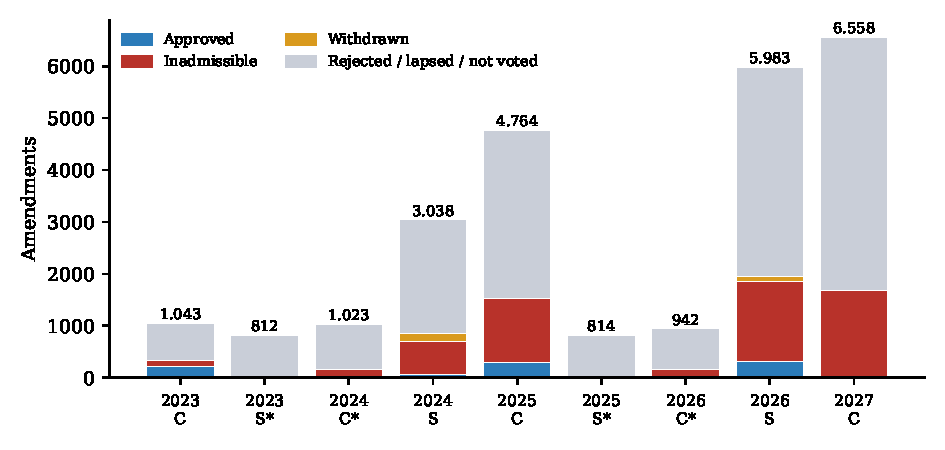
\includegraphics[width=\textwidth]{fig/fig1_counts.pdf}
\caption{Proposals by budget, chamber and outcome}\label{fig:counts}
\begin{minipage}{0.95\textwidth}\footnotesize \emph{Notes:} C = Chamber of Deputies, S = Senate; * second reading. The 2027 budget had not been voted in committee at the time of writing.\end{minipage}
\end{figure}

\section{Empirical strategy}\label{sec:strategy}

I build a balanced panel of 109 provinces (Valle d'Aosta, which has no list vote, is excluded) $\times$ 8 parties $\times$ 5 budgets, for 4,360 observations. The outcome $Y_{ipt}$ equals one if party $p$ tabled at least one local proposal naming province $i$ in budget $t$, in either chamber. I estimate linear probability models of the form
\begin{equation}
Y_{ipt} = \beta\, \text{Votes}_{ip} + \alpha_{pt} + \delta_{r(i)} + \varepsilon_{ipt},
\end{equation}
where $\text{Votes}_{ip}$ is the 2022 list vote share of party $p$ in province $i$, in units of ten percentage points, $\alpha_{pt}$ are party-by-budget fixed effects and $\delta_{r(i)}$ region fixed effects. Party-by-budget effects absorb differences in how many amendments each party tables each year; region effects absorb the North--South gradient in both votes and requests. In the most demanding specification I replace $\delta_{r(i)}$ with party-by-region effects $\delta_{pr(i)}$. This compares, for the same party, provinces of the same region where the party did better or worse in 2022. Standard errors are clustered by province \citep{cameron2015}. All coefficients are multiplied by 100 and read as percentage points.

I add two designs. The first replaces region effects with province-by-budget effects $\mu_{it}$, so that $\beta$ is identified only by comparing \emph{different parties in the same province and budget}: if party A received more votes than party B in province $i$, is A more likely than B to ask for money for $i$? Province-by-budget effects absorb every characteristic of the province that is common to all parties, including local needs, size, the presence of a crisis and the amount of money on offer. The second adds $\text{MP}_{ip}$, the number of party $p$'s deputies elected in province $i$. Deputies elected on lists are attached to multi-province constituencies, so I attribute each of them to the provinces of the constituency in proportion to the provinces' registered voters; group membership is taken from the current composition of the Chamber.\footnote{The attribution uses the 2022 constituency of each deputy listed by the Chamber in November 2026 and Ministry of the Interior data on registered voters by province and constituency. Deputies elected in single-member districts are attributed through their list constituency as well. Senators are not included, and changes of group during the legislature are not tracked in this variable.} The variable has mean 0.43 and standard deviation 0.80, and its correlation with vote share is 0.45. Because the number of deputies is itself an outcome of votes, the comparison is a decomposition (does the vote gradient run through elected legislators?) rather than a causal estimate.

The estimates are descriptive. Vote shares are not randomly assigned. Places where a party is strong may also have the local needs, such as industrial crises or infrastructure gaps, that its legislators choose to champion. The within-region design removes broad territorial differences but not province-specific shocks correlated with past votes. I therefore interpret $\beta$ as a description of where requests go, not as the causal effect of votes on requests.

\section{Results}\label{sec:results}

\subsection{Electoral strength and local requests}

Table~\ref{tab:main} reports the main estimates. Without geographic controls (column~1) ten points of vote share are associated with an increase of 11.7 points in the probability of a local request. Adding region fixed effects leaves the estimate essentially unchanged (column~2). With party-by-region effects the coefficient falls to 7.5 but remains precisely estimated (column~3): most of the association is between regions, but a meaningful part is within them. Columns 4--5 use the inverse hyperbolic sine of local requests per 100,000 residents and confirm the sign \citep{bellemare2020}. Figure~\ref{fig:bin} shows the corresponding binned scatter plots.

Columns 6--7 turn to approved local requests in the four budgets that have been voted. Approved requests are also more frequent where parties are strong across Italy (1.99 points, against a mean of 1.8\%), but the within-region coefficient is -0.13 with a standard error of 0.95. Legislators ask for their strongholds; the budget does not obviously deliver to them.

\begin{table}[htbp]\centering\footnotesize\setlength{\tabcolsep}{4pt}
\begin{threeparttable}
\caption{Electoral strength and local spending requests}\label{tab:main}
\begin{tabular}{lccccccc}
\toprule
 & (1) & (2) & (3) & (4) & (5) & (6) & (7) \\
Dependent variable & \multicolumn{3}{c}{Local request (0/1)} & \multicolumn{2}{c}{asinh(requests per 100k)} & \multicolumn{2}{c}{Approved request (0/1)} \\
\cmidrule(lr){2-4}\cmidrule(lr){5-6}\cmidrule(lr){7-8}
Vote share 2022 (10 pp) & $11.70^{***}$ & $12.17^{***}$ & $7.48^{**}$ & $0.068^{***}$ & $0.038^{**}$ & $1.99^{**}$ & $-0.13$ \\
 & (1.59) & (1.51) & (2.52) & (0.010) & (0.013) & (0.72) & (0.95) \\[3pt]
Party $\times$ budget FE & Yes & Yes & Yes & Yes & Yes & Yes & Yes \\
Region FE & No & Yes & -- & Yes & -- & Yes & -- \\
Party $\times$ region FE & No & No & Yes & No & Yes & No & Yes \\
Budgets & 2023--27 & 2023--27 & 2023--27 & 2023--27 & 2023--27 & 2023--26 & 2023--26 \\
Mean of dep. var. & 13.37 & 13.37 & 13.37 & 0.05 & 0.05 & 1.81 & 1.81 \\
Observations & 4,360 & 4,360 & 4,360 & 4,360 & 4,360 & 3,488 & 3,488 \\
\bottomrule
\end{tabular}
\begin{tablenotes}\footnotesize
\item \emph{Notes:} OLS. Unit: province $\times$ party $\times$ budget. Coefficients in columns 1--3 and 6--7 are in percentage points; means in percent. Standard errors clustered by province (109 clusters) in parentheses. $^{*}p<0.05$, $^{**}p<0.01$, $^{***}p<0.001$.
\end{tablenotes}
\end{threeparttable}
\end{table}

\begin{figure}[htbp]\centering
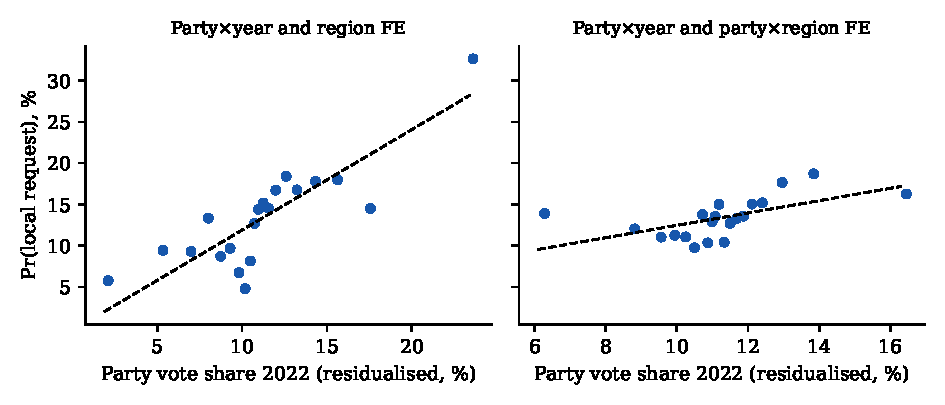
\includegraphics[width=\textwidth]{fig/fig2_binscatter.pdf}
\caption{Vote share in 2022 and the probability of a local request}\label{fig:bin}
\begin{minipage}{0.95\textwidth}\footnotesize \emph{Notes:} Twenty equal-sized bins of residualised vote share; dashed line: OLS slope from Table~\ref{tab:main}, columns 2 and 3.\end{minipage}
\end{figure}

\subsection{Comparing parties within the same province}

Table~\ref{tab:mp} reports the two additional designs. Column~1 replaces region effects with province-by-budget effects, so that only differences between parties within the same province and budget identify the coefficient. The estimate, 12.4 points (s.e.\ 1.6), is as large as the one with region effects. Whatever makes a province attract requests in a given year, from an industrial crisis to a flood, the party that is stronger there asks for money for it more often than the party that is weaker. Adding party-by-region effects as well (column~2) gives 8.6 points (s.e.\ 2.5), close to the within-region estimate of Table~\ref{tab:main}.

\subsection{Party strategy or legislator geography?}

A party that wins more votes in a province also elects more deputies from there, and those deputies may simply ask for money for home. Columns 3--6 of Table~\ref{tab:mp} add the number of the party's deputies attributed to the province. Across Italy (column~3, with region effects and log population) both variables matter: the vote-share coefficient falls only from 12.2 to 10.0, and each deputy adds 4.9 points. Within provinces (column~4) the picture is similar. Within regions (column~5) the deputy variable absorbs most of the gradient: the vote-share coefficient falls to 3.7 (s.e.\ 3.3) and each deputy adds 9.9 points (s.e.\ 1.3). Comparing provinces of the same region, a party asks for money where it has elected legislators, not where it is stronger as such.

This is consistent with the ``law of $1/n$'' of \citet{weingast1981}: each legislator internalises the benefit of spending in his or her constituency but only a small share of its cost. It is also consistent with the home bias documented for Italian transfers by \citet{carozzi2016}. The decomposition is not causal, because the number of deputies is itself a function of votes and of candidate selection.

\begin{table}[htbp]\centering\footnotesize\setlength{\tabcolsep}{4pt}
\begin{threeparttable}
\caption{Within-province comparisons and the geography of elected deputies}\label{tab:mp}
\begin{tabular}{lcccccc}
\toprule
 & (1) & (2) & (3) & (4) & (5) & (6) \\
\midrule
Vote share 2022 (10 pp) & $12.43^{***}$ & $8.57^{***}$ & $10.01^{***}$ & $11.25^{***}$ & $3.69$ & \\
 & (1.64) & (2.53) & (1.72) & (1.78) & (3.34) & \\
Deputies of the party elected in the province & & & $4.94^{***}$ & $2.66^{*}$ & $9.92^{***}$ & $5.77^{***}$ \\
 & & & (1.10) & (1.09) & (1.27) & (1.31) \\[3pt]
Party $\times$ budget FE & Yes & Yes & Yes & Yes & Yes & Yes \\
Province $\times$ budget FE & Yes & Yes & No & Yes & No & Yes \\
Region FE, log population & No & No & Yes & -- & No & -- \\
Party $\times$ region FE & No & Yes & No & No & Yes & No \\
Observations & 4,360 & 4,360 & 4,360 & 4,360 & 4,360 & 4,360 \\
\bottomrule
\end{tabular}
\begin{tablenotes}\footnotesize
\item \emph{Notes:} OLS; dependent variable: local request (0/1), mean 13.4\%. Coefficients in percentage points. Deputies: number of the party's current deputies elected in the list constituencies that include the province, weighted by the province's share of the constituency's registered voters (mean 0.43, s.d.\ 0.80). Standard errors clustered by province in parentheses. $^{*}p<0.05$, $^{**}p<0.01$, $^{***}p<0.001$.
\end{tablenotes}
\end{threeparttable}
\end{table}

\subsection{Budget by budget}

Figure~\ref{fig:byyear} and Table~\ref{tab:byyear} estimate the model separately for each budget. The cross-Italy coefficient is positive and significant every year. The within-region coefficient is positive in the first four budgets, between 8.4 and 14.3 points, though imprecise in single years. In the 2027 budget it is -4.4 (s.e. 6.3). Excluding 2027, the pooled within-region estimate rises to 10.4 (Table~\ref{tab:robust}). Whether 2027 marks a change, for instance as legislators approach the end of the legislature, or is noise, will become clearer with the Senate stage of that budget.

\begin{figure}[htbp]\centering
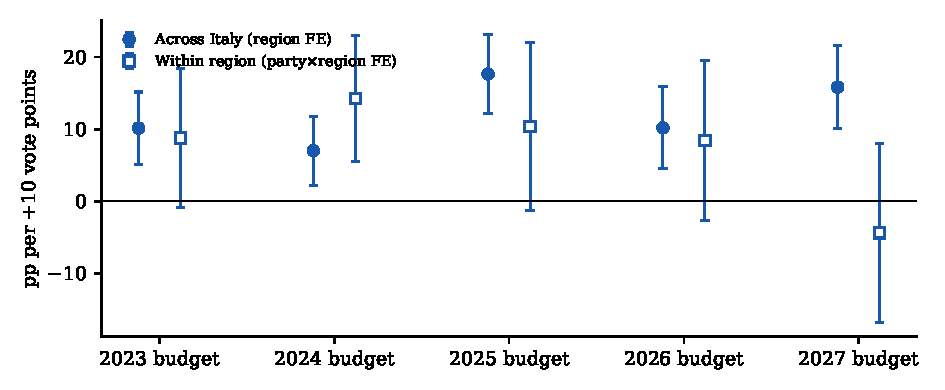
\includegraphics[width=\textwidth]{fig/fig3_byyear.pdf}
\caption{The vote--request gradient, budget by budget}\label{fig:byyear}
\begin{minipage}{0.95\textwidth}\footnotesize \emph{Notes:} Coefficients on 2022 vote share (10 pp) from separate regressions for each budget, with 95\% confidence intervals. Filled: party and region FE. Hollow: party $\times$ region FE.\end{minipage}
\end{figure}

\begin{table}[htbp]\centering\footnotesize\setlength{\tabcolsep}{4pt}
\begin{threeparttable}
\caption{Estimates by budget}\label{tab:byyear}
\begin{tabular}{lccccc}
\toprule
Budget & \multicolumn{2}{c}{Party and region FE} & \multicolumn{2}{c}{Party $\times$ region FE} & Mean (\%) \\
\midrule
2023 & $10.15^{***}$ & (2.55) & $8.79$ & (4.90) & 5.5 \\
2024 & $7.02^{**}$ & (2.43) & $14.25^{**}$ & (4.46) & 7.1 \\
2025 & $17.65^{***}$ & (2.79) & $10.35$ & (5.94) & 18.2 \\
2026 & $10.18^{***}$ & (2.90) & $8.40$ & (5.67) & 17.7 \\
2027 & $15.83^{***}$ & (2.92) & $-4.37$ & (6.32) & 18.3 \\
\bottomrule
\end{tabular}
\begin{tablenotes}\footnotesize
\item \emph{Notes:} Each row is a separate regression on 872 province--party observations; coefficients in percentage points, clustered standard errors in parentheses.
\end{tablenotes}
\end{threeparttable}
\end{table}

\subsection{Who targets strongholds?}

Table~\ref{tab:het} estimates the gradient separately for each party with region and budget fixed effects. The pooled result hides a sharp contrast. The three main opposition parties ask for money where they are strong: 26.8 points for the PD, 18.0 for the M5S and 74.0 for AVS, whose smaller vote shares mechanically produce larger coefficients. Fratelli d'Italia shows the opposite sign (-12.5, s.e. 4.3): within a region, its legislators table more local requests where the party did relatively worse in 2022. The estimates for the Lega and Forza Italia are negative but imprecise.

One interpretation is that governing and opposition parties use local amendments differently. For the opposition, an amendment is mainly a signal to its own voters, which is cheap and has a low chance of approval. For the senior governing party, whose requests have a real chance of passing, the amendment is an instrument to expand support where it is weaker, closer to the swing-voter logic of \citet{lindbeck1987} and \citet{dixit1996}. The evidence is suggestive: it rests on one large governing party and on cross-sectional variation in vote shares.

\begin{table}[htbp]\centering\footnotesize\setlength{\tabcolsep}{4pt}
\begin{threeparttable}
\caption{Heterogeneity by party}\label{tab:het}
\begin{tabular}{llccc}
\toprule
Party & Camp & Vote share (10 pp) & s.e. & Pairs with a request \\
\midrule
FdI & Majority & $-12.47^{**}$ & (4.31) & 67 \\
Lega & Majority & $-23.90$ & (13.08) & 81 \\
FI & Majority & $-3.38$ & (10.52) & 66 \\
Noi Moderati & Majority & $19.77$ & (17.06) & 14 \\
PD & Opposition & $26.80^{**}$ & (9.19) & 177 \\
M5S & Opposition & $17.97^{*}$ & (7.90) & 105 \\
AVS & Opposition & $73.97^{**}$ & (28.46) & 31 \\
Azione/IV & Opposition & $12.65$ & (18.84) & 42 \\
\bottomrule
\end{tabular}
\begin{tablenotes}\footnotesize
\item \emph{Notes:} Separate regressions for each party on 545 province--budget observations, with budget and region FE. Standard errors clustered by province.
\end{tablenotes}
\end{threeparttable}
\end{table}

Figure~\ref{fig:het} plots the same estimates together with the within-region ones. A single regression that interacts vote share with membership of the governing coalition gives a gradient of 22.7 points for opposition parties and a difference of -34.4 points (s.e.\ 10.3) for majority parties, again with party-by-region effects.

\begin{figure}[htbp]\centering
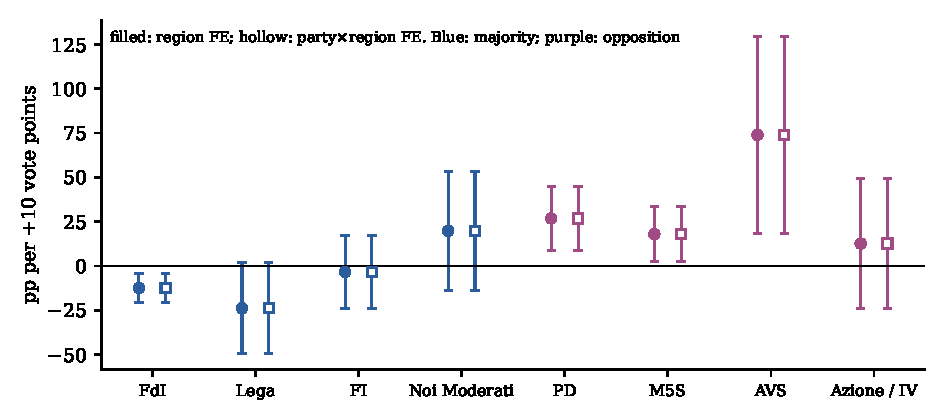
\includegraphics[width=\textwidth]{fig/fig7_het.pdf}
\caption{The vote--request gradient by party}\label{fig:het}
\begin{minipage}{0.95\textwidth}\footnotesize \emph{Notes:} Coefficients on 2022 vote share (10 pp) from separate regressions for each party, all five budgets, with 95\% confidence intervals. Filled: budget and region FE. Hollow: budget and party $\times$ region FE.\end{minipage}
\end{figure}

\subsection{Contested provinces and the pre-election budget}

Swing-voter models predict that parties target provinces where the election is close \citep{lindbeck1987,dixit1996}; models of electoral uncertainty predict that behaviour may change as the next election approaches \citep{alesina1990}. I define a province as contested if the 2022 gap between the centre-right (FdI, Lega, FI, Noi Moderati) and the centre-left (PD, AVS, +Europa) list votes is below the median, and interact vote share with this indicator and with the 2027 budget, with party-by-budget and party-by-region effects. The gradient is 3.6 points (s.e.\ 2.8) in safe provinces and 6.2 points higher (s.e.\ 2.3) in contested ones. The interaction with the 2027 budget is 5.0 (s.e.\ 3.3) and the triple interaction -0.6 (s.e.\ 2.4). Parties ask for money where they are strong, more so where the contest is open, and there is no clear sign that the pre-election budget is different; with a single pre-election budget this last comparison has little power.

\subsection{What gets approved}

I now move to the level of the single proposal and estimate the probability that a proposal is approved, using all proposals by majority and opposition legislators in the four first readings that have been voted (13,996 proposals, 499 first signatories). Table~\ref{tab:approval} reports linear probability models with chamber-by-budget fixed effects and standard errors clustered by first signatory.

Majority status is the dominant predictor. A majority proposal is 9.0 points more likely to pass, against an opposition base rate of 2.9\% (column~1); in raw terms, 12.4\% of majority proposals and 2.9\% of opposition proposals were approved. Majority proposals are also more often ruled inadmissible (30.3\% against 21.5\%), consistent with majority members tabling many narrow requests that the leadership later filters. Local proposals are not significantly more likely to pass once the signatory's camp is accounted for (column~2). Proposals co-signed by more legislators are more likely to pass and those asking for more than 100 million euro less likely (column~3). Comparing proposals by the same legislator (column~4), local requests are 3.2 points more likely to pass than the same legislator's general proposals. Figure~\ref{fig:approval} shows the majority--opposition gap budget by budget.

\begin{table}[htbp]\centering\footnotesize\setlength{\tabcolsep}{4pt}
\begin{threeparttable}
\caption{Probability that a proposal is approved}\label{tab:approval}
\begin{tabular}{lcccc}
\toprule
 & (1) & (2) & (3) & (4) \\
\midrule
Majority signatory & $9.00^{***}$ & $8.80^{***}$ & $8.78^{***}$ &  \\
 & (1.05) & (1.06) & (1.01) &  \\
Local proposal & & $1.66$ & $1.47$ & $3.16^{*}$ \\
 & & (1.21) & (1.29) & (1.36) \\
Majority $\times$ local & & $3.84$ & $3.70$ &  \\
 & & (3.56) & (3.53) &  \\
log(1 + co-signatories) & & & $2.79^{***}$ & $4.11^{***}$ \\
 & & & (0.67) & (0.78) \\
Request $\geq$ 100 million euro & & & $-4.45^{***}$ & $-4.31^{***}$ \\
 & & & (0.48) & (0.52) \\[3pt]
Chamber $\times$ budget FE & Yes & Yes & Yes & Yes \\
Topic FE & No & No & Yes & Yes \\
First-signatory FE & No & No & No & Yes \\
Observations & 13,996 & 13,996 & 13,996 & 13,996 \\
\bottomrule
\end{tabular}
\begin{tablenotes}\footnotesize
\item \emph{Notes:} Linear probability models; coefficients in percentage points. Sample: proposals by majority and opposition legislators in the first readings of the 2023--2026 budgets. Standard errors clustered by first signatory in parentheses. $^{*}p<0.05$, $^{**}p<0.01$, $^{***}p<0.001$.
\end{tablenotes}
\end{threeparttable}
\end{table}

\begin{figure}[htbp]\centering
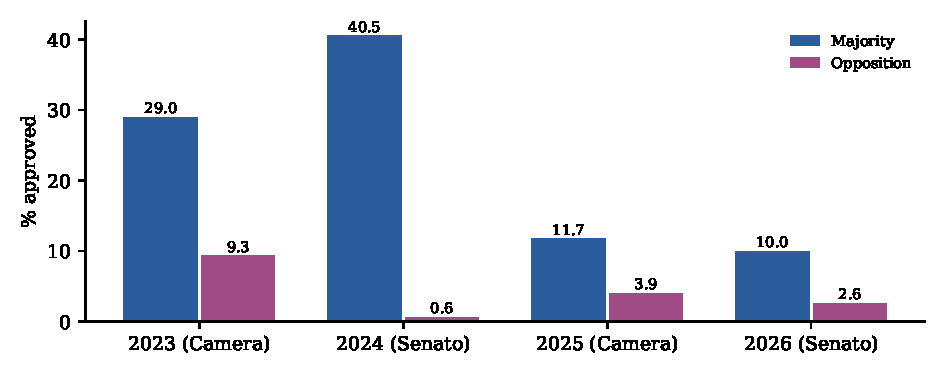
\includegraphics[width=\textwidth]{fig/fig5_approval.pdf}
\caption{Approval rates by camp, first readings}\label{fig:approval}
\end{figure}

\subsection{Where the majority premium arises}

The approval gap can arise at two stages: the admissibility ruling by the committee chair, or the vote, which in practice reflects the opinion of the government and of the rapporteurs. Figure~\ref{fig:stages} separates them. Majority proposals are \emph{less} likely to be ruled admissible: 69.7\% against 78.5\% for the opposition, -7.9 points (s.e.\ 1.5) with chamber-by-budget and topic effects. Local proposals are also more often inadmissible (-11.3 points, s.e.\ 2.4), mostly for extraneity of subject matter. Among admissible proposals, however, 17.8\% of majority proposals are approved against 3.7\% of opposition ones, a gap of 13.2 points (s.e.\ 1.4). The premium is created at the vote, not by the procedural filter. Selection is a concern: majority legislators may table more proposals that have already been negotiated with the government. Among approved local requests by majority parties, 7 were signed by FdI, 11 by the Lega and 11 by Forza Italia, so the smaller coalition partners obtain far more local approvals than their seat shares would suggest.

\begin{figure}[htbp]\centering
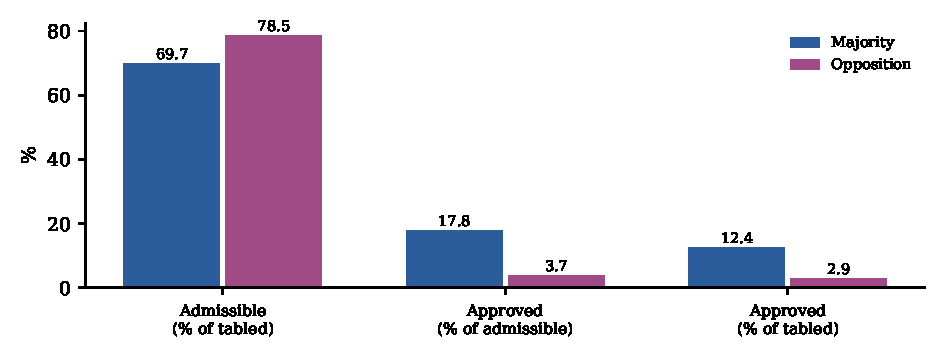
\includegraphics[width=\textwidth]{fig/fig8_stages.pdf}
\caption{Admissibility and approval by camp, first readings 2023--2026}\label{fig:stages}
\begin{minipage}{0.95\textwidth}\footnotesize \emph{Notes:} Proposals by majority and opposition legislators in the first readings of the 2023--2026 budgets. Admissible: not ruled inadmissible by the committee chair.\end{minipage}
\end{figure}

\subsection{The geography of requests}

Figure~\ref{fig:map} maps local requests per 100,000 residents over the whole legislature and the number of approved local requests. Requests are dense in Tuscany, Sicily and Apulia, regions where several opposition legislators are prolific signatories, and in provinces with industrial crises such as Taranto and Siracusa. Approved requests are much rarer: 73 province mentions spread over 38 provinces, led by Rome with nine.

\begin{figure}[htbp]\centering
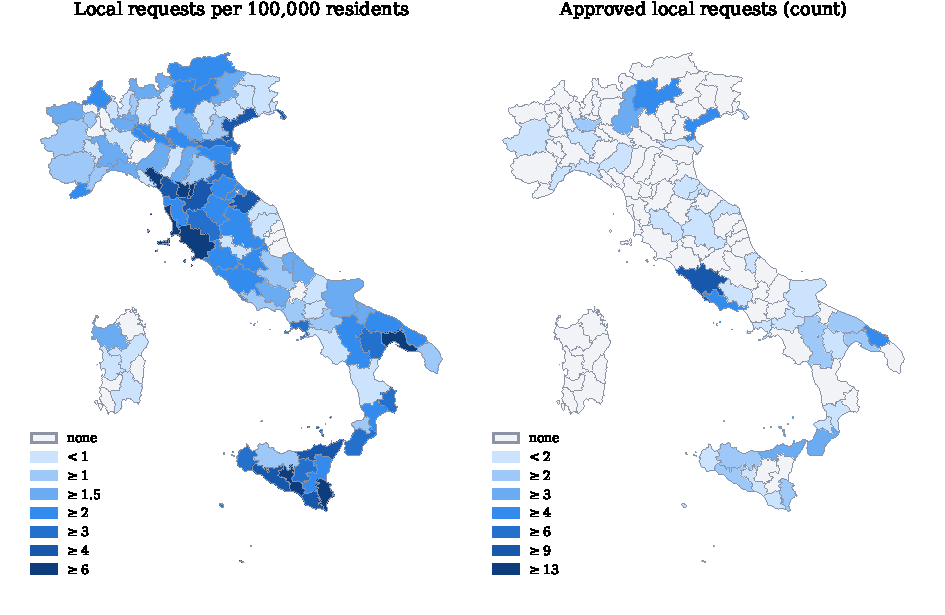
\includegraphics[width=\textwidth]{fig/fig4_map.pdf}
\caption{Local requests, 2023--2027 budgets}\label{fig:map}
\begin{minipage}{0.95\textwidth}\footnotesize \emph{Notes:} Proposals by legislators (excluding government and rapporteurs) naming a province or one of its municipalities, both chambers. A proposal naming several provinces counts once for each.\end{minipage}
\end{figure}

\section{Robustness}\label{sec:robust}

Table~\ref{tab:robust} re-estimates the two main specifications on different samples. The cross-Italy coefficient is positive and significant in every case. The within-region coefficient is positive and significant at the 5\% level in every sample, including each chamber separately, first readings only, and excluding the four largest metropolitan provinces. Excluding the 2023 budget, for which the Chamber published only flagged proposals, leaves the estimates unchanged. A logit model gives an average marginal effect of 7.8 points (s.e. 0.9) for the specification of column~2 of Table~\ref{tab:main}. Finally, I permute vote shares across provinces within each party, region and budget 300 times. A within-region coefficient as large as the observed one occurs in 0\% of permutations.


\paragraph{Specification curve.} To show that the result does not depend on a particular set of choices, I estimate every combination of three outcome definitions (any local request; local requests only, excluding multi-territorial ones; admissible requests only), four samples (both chambers; Chamber only; Senate only; first readings only), three sets of budgets for the pooled sample (all; excluding 2023; excluding 2027), four sets of fixed effects (region; party $\times$ region; province $\times$ budget; both) and two sets of provinces (all; excluding Rome, Milan, Naples and Turin), for 144 specifications \citep{simonsohn2020}. Figure~\ref{fig:spec} sorts the estimates. All are positive, ranging from 2.4 to 13.2 points, and 137 are significant at 5\%; the median is 8.5. The median estimate is 10.9 with region effects, 11.1 with province-by-budget effects, 6.4 with party-by-region effects and 7.5 with both: the comparisons within regions are the ones that shrink the gradient.

\paragraph{Counts.} A Poisson pseudo-maximum-likelihood model for the number of local requests \citep{santossilva2006}, with party-by-budget and region effects and log population, gives a coefficient of 0.66 (s.e.\ 0.08): ten points of vote share are associated with 1.93 times as many requests. With province-by-budget effects the coefficient is 0.68 (s.e.\ 0.11).

\begin{figure}[htbp]\centering
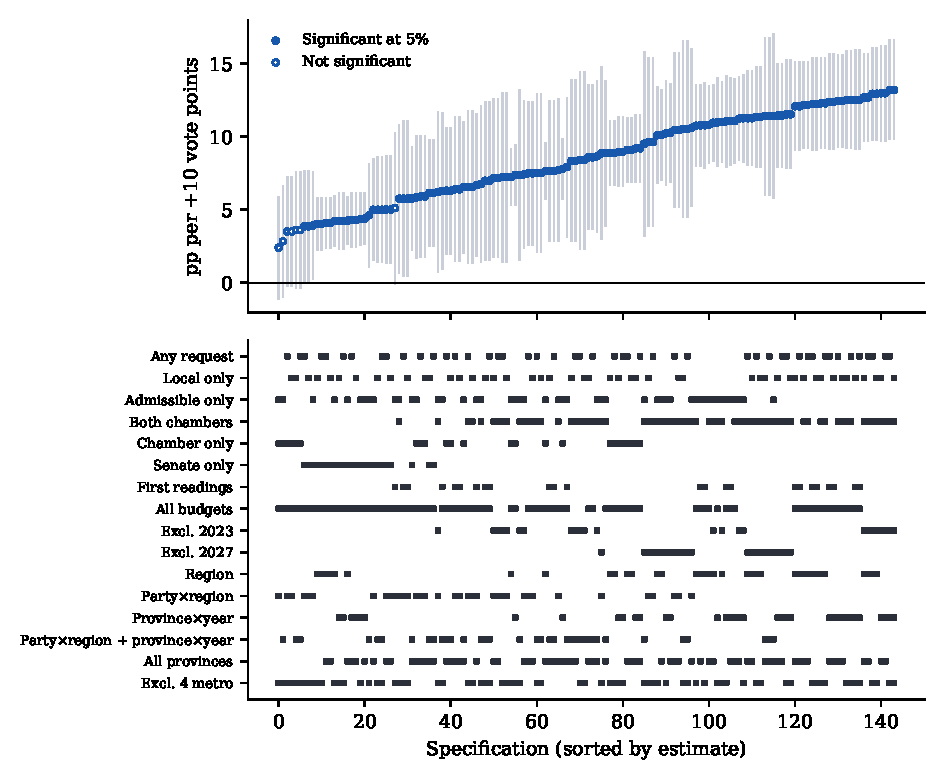
\includegraphics[width=\textwidth]{fig/fig6_spec.pdf}
\caption{Specification curve}\label{fig:spec}
\begin{minipage}{0.95\textwidth}\footnotesize \emph{Notes:} Upper panel: coefficient on 2022 vote share (10 pp) with 95\% confidence intervals, clustered by province, in 144 specifications sorted by size; filled points are significant at 5\%. Lower panel: the choices that define each specification. Chamber-only, Senate-only and first-reading samples use all five budgets.\end{minipage}
\end{figure}
\begin{table}[htbp]\centering\footnotesize\setlength{\tabcolsep}{4pt}
\begin{threeparttable}
\caption{Robustness}\label{tab:robust}
\begin{tabular}{lcccc}
\toprule
 & \multicolumn{2}{c}{Region FE} & \multicolumn{2}{c}{Party $\times$ region FE} \\
\cmidrule(lr){2-3}\cmidrule(lr){4-5}
Sample & Coef. & s.e. & Coef. & s.e. \\
\midrule
Baseline (Table 2, cols. 2--3) & $12.17^{***}$ & (1.51) & $7.48^{**}$ & (2.52) \\
Chamber of Deputies only & $9.08^{***}$ & (1.13) & $5.90^{**}$ & (2.13) \\
Senate only & $4.09^{***}$ & (0.88) & $5.00^{**}$ & (1.87) \\
First readings only & $12.06^{***}$ & (1.56) & $6.38^{*}$ & (2.54) \\
Excluding 2023 (partial data) & $12.67^{***}$ & (1.55) & $7.16^{**}$ & (2.77) \\
Excluding 2027 (not yet voted) & $11.25^{***}$ & (1.66) & $10.45^{***}$ & (2.70) \\
Excluding Rome, Milan, Naples, Turin & $12.27^{***}$ & (1.59) & $6.53^{*}$ & (2.66) \\
\bottomrule
\end{tabular}
\begin{tablenotes}\footnotesize
\item \emph{Notes:} All regressions include party $\times$ budget FE. Dependent variable: local request (0/1). Coefficients on 2022 vote share (10 pp), in percentage points; standard errors clustered by province.
\end{tablenotes}
\end{threeparttable}
\end{table}

\section{Discussion and conclusion}\label{sec:concl}

Members of the Italian Parliament ask for local money where their party is strong. The pattern is stable across five budgets, both chambers and 144 specifications, and it holds when parties are compared within the same province and budget. Within regions it runs through the geography of elected deputies, which points to individual legislators claiming resources for their own constituencies rather than to a centrally planned party strategy. It is driven by the opposition, while the senior governing party leans towards provinces where it is weaker. Whether a request becomes law depends overwhelmingly on whether the signatory sits in the majority; the premium arises at the vote, not at the admissibility stage, and approved local money does not track electoral strength within regions.
Proponents of local spending often defend it as an investment that pays for itself through its effects on the local economy. The evidence on local fiscal multipliers does not support that argument as a general rule. Estimates based on Italian provinces find output multipliers of about 1.5 for public works \citep{acconcia2014}, and the cross-regional literature finds multipliers of a similar size \citep{chodorowreich2019}. These are relative effects that partly reflect resources moved from elsewhere in the country, and a multiplier of 1.5 is far from what would be needed for spending to finance itself through tax revenue. A text search of the dataset finds no local amendment that quantifies such an effect.


Three caveats apply. The analysis is descriptive, and local needs correlated with past votes may explain part of the gradient. Places and sums are extracted automatically from legal texts; I validated the procedure on samples but errors remain, and I avoid relying on euro amounts. The data are not homogeneous across years: the 2023 Chamber file covers flagged proposals only, second readings are mostly symbolic, and the 2027 budget is still under examination.

The dataset opens several avenues. The approved amendments can be linked to the financial effects certified by the parliamentary budget services to measure how much of the final budget is shaped in Parliament. The attribution of deputies to provinces can be refined with single-member districts, senators and the place of birth or residence of each legislator, and the scheduled calendar of municipal elections offers a source of variation in the timing of local incentives that is plausibly unrelated to budget politics. The Senate stage of the 2027 budget will show whether the weaker within-region pattern of that year persists.

\section*{Data availability}\label{sec:avail}\sloppy
The dataset and a replication package (R code that reproduces every table and figure from the CSV files) have been prepared and are available from the author on request; they will be made public upon publication. All primary sources are public on the websites of the Chamber of Deputies, the Senate of the Republic, the Ministry of the Interior and ISTAT.

\begin{thebibliography}{99}\small
\bibitem[Acconcia et~al.(2014)]{acconcia2014} Acconcia, A., Corsetti, G., and Simonelli, S. (2014). Mafia and public spending: Evidence on the fiscal multiplier from a quasi-experiment. \emph{American Economic Review}, 104(7), 2185--2209.
\bibitem[Alesina and Tabellini(1990)]{alesina1990} Alesina, A., and Tabellini, G. (1990). A positive theory of fiscal deficits and government debt. \emph{Review of Economic Studies}, 57(3), 403--414.
\bibitem[Ansolabehere and Snyder(2006)]{ansolabehere2006} Ansolabehere, S., and Snyder, J.~M. (2006). Party control of state government and the distribution of public expenditures. \emph{Scandinavian Journal of Economics}, 108(4), 547--569.
\bibitem[Bellemare and Wichman(2020)]{bellemare2020} Bellemare, M.~F., and Wichman, C.~J. (2020). Elasticities and the inverse hyperbolic sine transformation. \emph{Oxford Bulletin of Economics and Statistics}, 82(1), 50--61.
\bibitem[Berry et~al.(2010)]{berry2010} Berry, C.~R., Burden, B.~C., and Howell, W.~G. (2010). The president and the distribution of federal spending. \emph{American Political Science Review}, 104(4), 783--799.
\bibitem[Bracco et~al.(2015)]{bracco2015} Bracco, E., Lockwood, B., Porcelli, F., and Redoano, M. (2015). Intergovernmental grants as signals and the alignment effect: Theory and evidence. \emph{Journal of Public Economics}, 123, 78--91.
\bibitem[Brollo and Nannicini(2012)]{brollo2012} Brollo, F., and Nannicini, T. (2012). Tying your enemy's hands in close races: The politics of federal transfers in Brazil. \emph{American Political Science Review}, 106(4), 742--761.
\bibitem[Cameron and Miller(2015)]{cameron2015} Cameron, A.~C., and Miller, D.~L. (2015). A practitioner's guide to cluster-robust inference. \emph{Journal of Human Resources}, 50(2), 317--372.
\bibitem[Carozzi and Repetto(2016)]{carozzi2016} Carozzi, F., and Repetto, L. (2016). Sending the pork home: Birth town bias in transfers to Italian municipalities. \emph{Journal of Public Economics}, 134, 42--52.
\bibitem[Chodorow-Reich(2019)]{chodorowreich2019} Chodorow-Reich, G. (2019). Geographic cross-sectional fiscal spending multipliers: What have we learned? \emph{American Economic Journal: Economic Policy}, 11(2), 1--34.
\bibitem[Cox and McCubbins(1986)]{cox1986} Cox, G.~W., and McCubbins, M.~D. (1986). Electoral politics as a redistributive game. \emph{Journal of Politics}, 48(2), 370--389.
\bibitem[Dixit and Londregan(1996)]{dixit1996} Dixit, A., and Londregan, J. (1996). The determinants of success of special interests in redistributive politics. \emph{Journal of Politics}, 58(4), 1132--1155.
\bibitem[Golden and Picci(2008)]{golden2008} Golden, M.~A., and Picci, L. (2008). Pork-barrel politics in postwar Italy, 1953--94. \emph{American Journal of Political Science}, 52(2), 268--289.
\bibitem[Levitt and Snyder(1997)]{levitt1997} Levitt, S.~D., and Snyder, J.~M. (1997). The impact of federal spending on House election outcomes. \emph{Journal of Political Economy}, 105(1), 30--53.
\bibitem[Lindbeck and Weibull(1987)]{lindbeck1987} Lindbeck, A., and Weibull, J.~W. (1987). Balanced-budget redistribution as the outcome of political competition. \emph{Public Choice}, 52(3), 273--297.
\bibitem[Mayhew(1974)]{mayhew1974} Mayhew, D.~R. (1974). \emph{Congress: The Electoral Connection}. New Haven: Yale University Press.
\bibitem[Persson and Tabellini(1999)]{perssontabellini1999} Persson, T., and Tabellini, G. (1999). Political economics and macroeconomic policy. In J.~B. Taylor and M.~Woodford (eds.), \emph{Handbook of Macroeconomics}, Vol.~1C, ch.~22, 1397--1482. Amsterdam: Elsevier.
\bibitem[Santos Silva and Tenreyro(2006)]{santossilva2006} Santos Silva, J.~M.~C., and Tenreyro, S. (2006). The log of gravity. \emph{Review of Economics and Statistics}, 88(4), 641--658.
\bibitem[Simonsohn et~al.(2020)]{simonsohn2020} Simonsohn, U., Simmons, J.~P., and Nelson, L.~D. (2020). Specification curve analysis. \emph{Nature Human Behaviour}, 4(11), 1208--1214.
\bibitem[Weingast et~al.(1981)]{weingast1981} Weingast, B.~R., Shepsle, K.~A., and Johnsen, C. (1981). The political economy of benefits and costs: A neoclassical approach to distributive politics. \emph{Journal of Political Economy}, 89(4), 642--664.
\end{thebibliography}
\end{document}
